\documentclass[12pt,]{article}
\usepackage[left=1in,top=1in,right=1in,bottom=1in]{geometry}
\newcommand*{\authorfont}{\fontfamily{phv}\selectfont}
\usepackage[]{libertine}


  \usepackage[T1]{fontenc}
  \usepackage[utf8]{inputenc}




\usepackage{abstract}
\renewcommand{\abstractname}{}    % clear the title
\renewcommand{\absnamepos}{empty} % originally center

\renewenvironment{abstract}
 {{%
    \setlength{\leftmargin}{0mm}
    \setlength{\rightmargin}{\leftmargin}%
  }%
  \relax}
 {\endlist}

\makeatletter
\def\@maketitle{%
  \newpage
%  \null
%  \vskip 2em%
%  \begin{center}%
  \let \footnote \thanks
    {\fontsize{18}{20}\selectfont\raggedright  \setlength{\parindent}{0pt} \@title \par}%
}
%\fi
\makeatother




\setcounter{secnumdepth}{0}

\usepackage{color}
\usepackage{fancyvrb}
\newcommand{\VerbBar}{|}
\newcommand{\VERB}{\Verb[commandchars=\\\{\}]}
\DefineVerbatimEnvironment{Highlighting}{Verbatim}{commandchars=\\\{\}}
% Add ',fontsize=\small' for more characters per line
\usepackage{framed}
\definecolor{shadecolor}{RGB}{248,248,248}
\newenvironment{Shaded}{\begin{snugshade}}{\end{snugshade}}
\newcommand{\AlertTok}[1]{\textcolor[rgb]{0.94,0.16,0.16}{#1}}
\newcommand{\AnnotationTok}[1]{\textcolor[rgb]{0.56,0.35,0.01}{\textbf{\textit{#1}}}}
\newcommand{\AttributeTok}[1]{\textcolor[rgb]{0.77,0.63,0.00}{#1}}
\newcommand{\BaseNTok}[1]{\textcolor[rgb]{0.00,0.00,0.81}{#1}}
\newcommand{\BuiltInTok}[1]{#1}
\newcommand{\CharTok}[1]{\textcolor[rgb]{0.31,0.60,0.02}{#1}}
\newcommand{\CommentTok}[1]{\textcolor[rgb]{0.56,0.35,0.01}{\textit{#1}}}
\newcommand{\CommentVarTok}[1]{\textcolor[rgb]{0.56,0.35,0.01}{\textbf{\textit{#1}}}}
\newcommand{\ConstantTok}[1]{\textcolor[rgb]{0.00,0.00,0.00}{#1}}
\newcommand{\ControlFlowTok}[1]{\textcolor[rgb]{0.13,0.29,0.53}{\textbf{#1}}}
\newcommand{\DataTypeTok}[1]{\textcolor[rgb]{0.13,0.29,0.53}{#1}}
\newcommand{\DecValTok}[1]{\textcolor[rgb]{0.00,0.00,0.81}{#1}}
\newcommand{\DocumentationTok}[1]{\textcolor[rgb]{0.56,0.35,0.01}{\textbf{\textit{#1}}}}
\newcommand{\ErrorTok}[1]{\textcolor[rgb]{0.64,0.00,0.00}{\textbf{#1}}}
\newcommand{\ExtensionTok}[1]{#1}
\newcommand{\FloatTok}[1]{\textcolor[rgb]{0.00,0.00,0.81}{#1}}
\newcommand{\FunctionTok}[1]{\textcolor[rgb]{0.00,0.00,0.00}{#1}}
\newcommand{\ImportTok}[1]{#1}
\newcommand{\InformationTok}[1]{\textcolor[rgb]{0.56,0.35,0.01}{\textbf{\textit{#1}}}}
\newcommand{\KeywordTok}[1]{\textcolor[rgb]{0.13,0.29,0.53}{\textbf{#1}}}
\newcommand{\NormalTok}[1]{#1}
\newcommand{\OperatorTok}[1]{\textcolor[rgb]{0.81,0.36,0.00}{\textbf{#1}}}
\newcommand{\OtherTok}[1]{\textcolor[rgb]{0.56,0.35,0.01}{#1}}
\newcommand{\PreprocessorTok}[1]{\textcolor[rgb]{0.56,0.35,0.01}{\textit{#1}}}
\newcommand{\RegionMarkerTok}[1]{#1}
\newcommand{\SpecialCharTok}[1]{\textcolor[rgb]{0.00,0.00,0.00}{#1}}
\newcommand{\SpecialStringTok}[1]{\textcolor[rgb]{0.31,0.60,0.02}{#1}}
\newcommand{\StringTok}[1]{\textcolor[rgb]{0.31,0.60,0.02}{#1}}
\newcommand{\VariableTok}[1]{\textcolor[rgb]{0.00,0.00,0.00}{#1}}
\newcommand{\VerbatimStringTok}[1]{\textcolor[rgb]{0.31,0.60,0.02}{#1}}
\newcommand{\WarningTok}[1]{\textcolor[rgb]{0.56,0.35,0.01}{\textbf{\textit{#1}}}}



\title{CSC8631 Coursework Assignment  }
 



\author{\Large Mariela Ayu Prasetyo
(210407835)\vspace{0.05in} \newline\normalsize\emph{Newcastle
University}  }


\date{}

\usepackage{titlesec}

\titleformat*{\section}{\normalsize\bfseries}
\titleformat*{\subsection}{\normalsize\itshape}
\titleformat*{\subsubsection}{\normalsize\itshape}
\titleformat*{\paragraph}{\normalsize\itshape}
\titleformat*{\subparagraph}{\normalsize\itshape}


\usepackage{natbib}
\bibliographystyle{apsr}
\usepackage[strings]{underscore} % protect underscores in most circumstances



\newtheorem{hypothesis}{Hypothesis}
\usepackage{setspace}


% set default figure placement to htbp
\makeatletter
\def\fps@figure{htbp}
\makeatother

\usepackage{hyperref}
\usepackage{array}
\usepackage{caption}
\usepackage{graphicx}
\usepackage{siunitx}
\usepackage{multirow}
\usepackage{hhline}
\usepackage{calc}
\usepackage{tabularx}
\usepackage{fontawesome}
\usepackage[para,online,flushleft]{threeparttable}

% move the hyperref stuff down here, after header-includes, to allow for - \usepackage{hyperref}

\makeatletter
\@ifpackageloaded{hyperref}{}{%
\ifxetex
  \PassOptionsToPackage{hyphens}{url}\usepackage[setpagesize=false, % page size defined by xetex
              unicode=false, % unicode breaks when used with xetex
              xetex]{hyperref}
\else
  \PassOptionsToPackage{hyphens}{url}\usepackage[draft,unicode=true]{hyperref}
\fi
}

\@ifpackageloaded{color}{
    \PassOptionsToPackage{usenames,dvipsnames}{color}
}{%
    \usepackage[usenames,dvipsnames]{color}
}
\makeatother
\hypersetup{breaklinks=true,
            bookmarks=true,
            pdfauthor={Mariela Ayu Prasetyo (210407835) (Newcastle
University)},
             pdfkeywords = {},  
            pdftitle={CSC8631 Coursework Assignment},
            colorlinks=true,
            citecolor=blue,
            urlcolor=blue,
            linkcolor=magenta,
            pdfborder={0 0 0}}
\urlstyle{same}  % don't use monospace font for urls

% Add an option for endnotes. -----


% add tightlist ----------
\providecommand{\tightlist}{%
\setlength{\itemsep}{0pt}\setlength{\parskip}{0pt}}

% add some other packages ----------

% \usepackage{multicol}
% This should regulate where figures float
% See: https://tex.stackexchange.com/questions/2275/keeping-tables-figures-close-to-where-they-are-mentioned
\usepackage[section]{placeins}


\begin{document}
	
% \pagenumbering{arabic}% resets `page` counter to 1 
%    

% \maketitle

{% \usefont{T1}{pnc}{m}{n}
\setlength{\parindent}{0pt}
\thispagestyle{plain}
{\fontsize{18}{20}\selectfont\raggedright 
\maketitle  % title \par  

}

{
   \vskip 13.5pt\relax \normalsize\fontsize{11}{12} 
\textbf{\authorfont Mariela Ayu Prasetyo
(210407835)} \hskip 15pt \emph{\small Newcastle University}   

}

}






\vskip -8.5pt


 % removetitleabstract

\noindent  

\hypertarget{introduction}{%
\section{Introduction}\label{introduction}}

This report aims to discuss and report any findings to the CSC8631
coursework assignment regarding exploratory data analysis in learning
analytics. The students were provided with dataset from FutureLearn
MOOC. We are then asked to provide any valuable or non-valuable insights
while following the best-practice development explained thoroughly via
the teaching resources available. To ensure we are following the
data-driven process throughout the project, we will also be adhering to
the CRISP-DM methodology. Lastly, we will wrap up with a conclusion
regarding the overall findings.

\hypertarget{business-understanding}{%
\section{Business Understanding}\label{business-understanding}}

The first step of CRISP-DM is the \emph{Business Understanding} step,
where we try to understand what the business wants to solve. In this
particular project, we are given the data set regarding a course in the
FutureLearn MOOC platform. Just like a real-life face-to-face class, we
want to find out whether students are involved in the class or not and
how many students continue to participate until the end of the semester.
We are also interested in finding out how many students leave the course
and, naturally, their reason for doing so. Next, we want to find out
which topics students are most interested to learn about. Lastly, we
also want to check what device students watch most of the video from.
Thus, we want to check the correlation between the video views and the
device form. After formulating the previous problems into a sentence, we
come up with the following precise questions:

\begin{itemize}
\tightlist
\item
  Is the students in the course highly engaged?\\
  The results can gain insight into whether further action to increase
  the engagement rate is necessary or not.
\item
  How many students and what causes students to leave the course?\\
  The results can determine the primary cause for students leaving and
  what to change in the future course run.
\item
  Which topic interests students the most?\\
  The results can be implemented in the future course run when
  determining the course topic.
\item
  Is there any correlation between the video views and the device
  form?\\
  The results can gain insight when designing course videos in the
  future course run.
\end{itemize}

\hypertarget{data-understanding-and-data-preparation}{%
\section{Data Understanding and Data
Preparation}\label{data-understanding-and-data-preparation}}

After formulating the questions, we move on to the \emph{Data
Understanding} and \emph{Data Preparation} part, where we focus on
understanding and formatting the data that assist the business tasks
defined in \emph{Business Understanding}. This phase will consist of:

\begin{itemize}
\item
  Describe data: In this part, we try to understand and describe the
  data in a short description. We can do this by examining the data
  format, the number of rows and columns, and the features that are
  accessible. We are also going to explain which data we are going to
  pick.
\item
  Exploring the data: In this section, we are trying to analyse the
  relationship between data and visualise the data. The conclusion and
  visualisation of the data exploration should support and verify the
  business question defined previously. We will tailor the data by
  selecting, cleaning, integrating, and formatting it.
\end{itemize}

\hypertarget{describe-data}{%
\subsection{Describe Data}\label{describe-data}}

Firstly, we are given the data set regarding an online course from the
FutureLearn MOOC platform. The data set consists of several files from
run 1 to run 7. Each run may consist of the following data in the .csv
form (the number inside the bracket denotes how many variables are there
in the file):

\begin{itemize}
\tightlist
\item
  archetype survey response (4)
\item
  enrolments (13)
\item
  leaving survey response (8)
\item
  question response (10)
\item
  step activity (6)
\item
  team members (5)
\item
  video stats (28)
\item
  weekly sentiment survey response (4)
\end{itemize}

\noindent Each of the files consists of different rows (entries), and
all the columns (variables) are stored in a chr and num format.\\
\hfill\break In this project, we will consider several files related to
our observations only. The files are :

\begin{itemize}
\tightlist
\item
  cyber-security-*\_enrolments.csv (run 1 to 7)\\
  We are going to use these files to answer question number one
\item
  cyber-security-*\_leaving-survey-responses.csv (run 1 to 7)\\
  We are going to use these files to answer question number two
\item
  cyber-security-*\_video-stats.csv (run 3 to 7)\\
  We are going to use these files to answer questions number three and
  four
\end{itemize}

\noindent Other files will be dropped since they are unrelated to our
questions.

\hypertarget{exploring-the-data}{%
\subsection{Exploring the Data}\label{exploring-the-data}}

In this section, we will begin to explore the given data set. In
particular, we want to explore the area where the solution will support
the problem defined in the \emph{Business Understanding} part. There are
three questions, and we will explore them one by one. For the graph
result, we will include and discuss them in the \emph{Modeling} and
\emph{Evaluation} phase.

\hypertarget{question-1}{%
\subsubsection{Question 1}\label{question-1}}

\textbf{What is the participation rate of the students?}\\
\hfill\break We want to analyse whether students are highly engaged in
the course for the first question. There are many ways to check this,
but we will review the total participation rate. We will focus on how
many percentages of students fully participated and finished the
material of the classes. We will also check the duration of the
completion for each student, and we can do this by checking the
enrolments.csv provided in the data set.\\
\hfill\break Firstly, we will do some data pre-processing for part one,
and the corresponding script is enrolments.R located in the /munge
folder. We read and store each run of enrolments in a single variable
for later use. After that, we begin processing our data, and the
corresponding script is fully\_participated.R is located in the /src
folder. We start by subsetting the students who fully participated in
the course (there are entries for the fully\_participated columns in the
csv data). Then, we convert the enrolled\_at and fully\_participated
variables of each run from string format to date format to calculate the
duration later using the difftime function. We convert it by using the
as.Date function. It is also worth mentioning that we store the code
inside a function for a more effective writing process for the
converting and calculating duration part.\\
\hfill\break After converting it, we calculate the duration between the
fully\_participated\_at and enrolled\_at and store it in a new variable.
We also remove entries or outliers for each run where the period exceeds
365 days or one year. Lastly, we calculate the percentage of students
who fully participated in the course proportion to the overall
enrollment for each run.

\hypertarget{question-2}{%
\subsubsection{Question 2}\label{question-2}}

\textbf{How many students and what causes students to leave the
course?}\\
\hfill\break For the second question, we want to analyse how many
students leave the course, what time they quit, and why. Same as before,
we will begin by pre-processing the data from leaving survey responses.
It is worth mentioning that we assume people who formally quit the
course are all required to fill the survey, so the number of students
who formally leave the class is equal to the number of the survey
entries.\\
\hfill\break We read the file and store each run data in a variable
similar to before. The corresponding pre-processing script is leaving.R
located in /munge folder. We can then move on to the processing script,
leaving\_reason.R, located in the/src folder. We begin by merging the
enrolment and leaving data to extract the enrolment\_at column. The
column later will be used to calculate the duration between the starting
and leaving date. Then, we drop the columns unrelated to our
observations, such as id, last\_completed\_step\_at, etc.\\
\hfill\break Like before, we convert the date from string format to date
format and calculate the duration between the starting and leaving dates
using the difftime function. We also compute how many percentages of
students formally quit the course. Lastly, we bind the data and quantify
the students' leaving reason for easier graphing. We will then calculate
the number of times each cause got picked. We will discuss the result in
the discussion area for a more detailed explanation.

\hypertarget{question-3}{%
\subsubsection{Question 3}\label{question-3}}

\textbf{Which topic interests students the most?}\\
\hfill\break For the third question, we will see which topic interests
students the most through the video viewing status provided in the
video-stats.csv. In particular, we will check variable total views and
viewed\_onehundred\_percent. Then, we will discuss the results in the
discussion section. We will begin by pre-processing the data first, with
the script video.R located in the /munge folder.\\
\hfill\break After the pre-processing phase, we can process the data
(video\_topic.R located in/src folder). We will keep only the variables
or columns related to our observations for each run. Those variables are
step position, title, total\_views, and viewed\_onehundred\_percent.
Next, we will index the data according to the run and bind them together
to simplify the graphing process. To get an accurate x-axis, we will
convert the step\_position from numeric format into the string format.

\hypertarget{question-4}{%
\subsubsection{Question 4}\label{question-4}}

\textbf{Is there any correlation between the number of views and the
device form?}\\
\hfill\break We want to check the correlation between the total number
of views and the device form for problem four. The code is in the
video\_topic.R located in the /src folder. We will only keep the related
variables, which are video\_duration, total\_views,
viewed\_onehundred\_percent, desktop\_device\_percentage,
mobile\_device\_percentage, and tablet\_device\_percentage. Console and
tv entries will be discarded since it only amounts to a little. After
subsetting the data, we compute the correlation using the cor function.
We will then store the result in a variable and discuss the result in
the next phase.

\begin{Shaded}
\begin{Highlighting}[]
\NormalTok{cor\_res }\OtherTok{\textless{}{-}} \FunctionTok{cor}\NormalTok{(video\_cor)}
\end{Highlighting}
\end{Shaded}

\hypertarget{modeling-and-evaluation}{%
\section{Modeling and Evaluation}\label{modeling-and-evaluation}}

This section combines two different phases for a more straightforward
reading format. For the modeling part, we will graph our findings
question by question, and for the evaluation, we will discuss any
results we can derive from the graph.

\hypertarget{question-1-1}{%
\subsubsection{Question 1}\label{question-1-1}}

\textbf{What is the participation rate of the students?}\\
\hfill\break For the first question, we want to analyse whether students
are highly engaged in the course by checking the percentages of students
who fully participated and finished the material of the classes.
Additionally, the duration of the completion for each student will also
be limited. After preparing the data in the previous phase, we can now
plot the graph.\\
\hfill\break For the first graph, we will graph using ggplot2 to plot
the completion duration against each student's starting date in each
run.

\begin{Shaded}
\begin{Highlighting}[]
\CommentTok{\# Insert plot 1}
\NormalTok{graph1}
\end{Highlighting}
\end{Shaded}

\begin{center}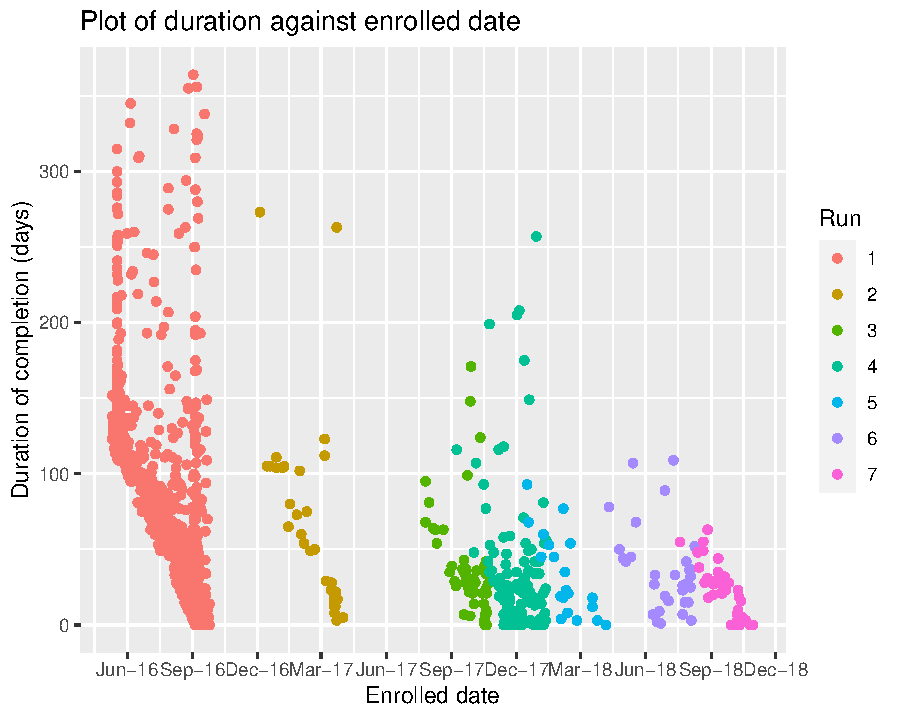
\includegraphics{report_files/figure-latex/unnamed-chunk-3-1} \end{center}

For the second graph, we will include the percentage of students who
fully participated in the course in proportion to the overall enrollment
for each run.

\begin{Shaded}
\begin{Highlighting}[]
\CommentTok{\# Insert plot 2}
\NormalTok{graph2}
\end{Highlighting}
\end{Shaded}

\begin{center}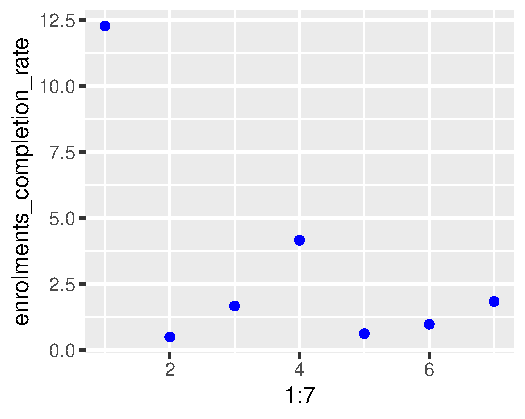
\includegraphics{report_files/figure-latex/unnamed-chunk-4-1} \end{center}

\hypertarget{discussion}{%
\subsubsection{Discussion}\label{discussion}}

In graph 1, we can see that duration of students completing the courses
varies but is primarily concentrated in 0 to 150 days. We can also see
that the number of people who fully participated in the class decreases
for each run. This means that the class gets less engaging as time goes
by, and different approaches are needed to boost the engagement rate of
the students. Additionally, the graph shows runs that open in the latter
half of the year gain more enrollment than those in the first half of
the year. This pattern could be considered when opening a new run in the
future.\\
\hfill\break Graph 2 shows the percentage of students who fully
participated in proportion to the overall enrolments against each run.
We can see that it peaked at 12.5\% for run one and stays under 5\%
after that. It confirms the statement before that the students who fully
participated decreased for each run. The overall findings suggest that
full participation or engagement seems to be pretty low; maybe it can be
considered in the future.

\hypertarget{question-2-1}{%
\subsubsection{Question 2}\label{question-2-1}}

\textbf{How many students and what causes students to leave the
course?}\\
\hfill\break For the second question, we want to evaluate the number of
students leaving the course, the time they quit, and why. We will now
plot the graph using library ggplot2 and the data prepared in the phase
before.\\
\hfill\break Graph 3 will demonstrate the duration from starting date
until leaving date against the leaving date.

\begin{Shaded}
\begin{Highlighting}[]
\CommentTok{\# Insert plot 3}
\NormalTok{graph3}
\end{Highlighting}
\end{Shaded}

\begin{center}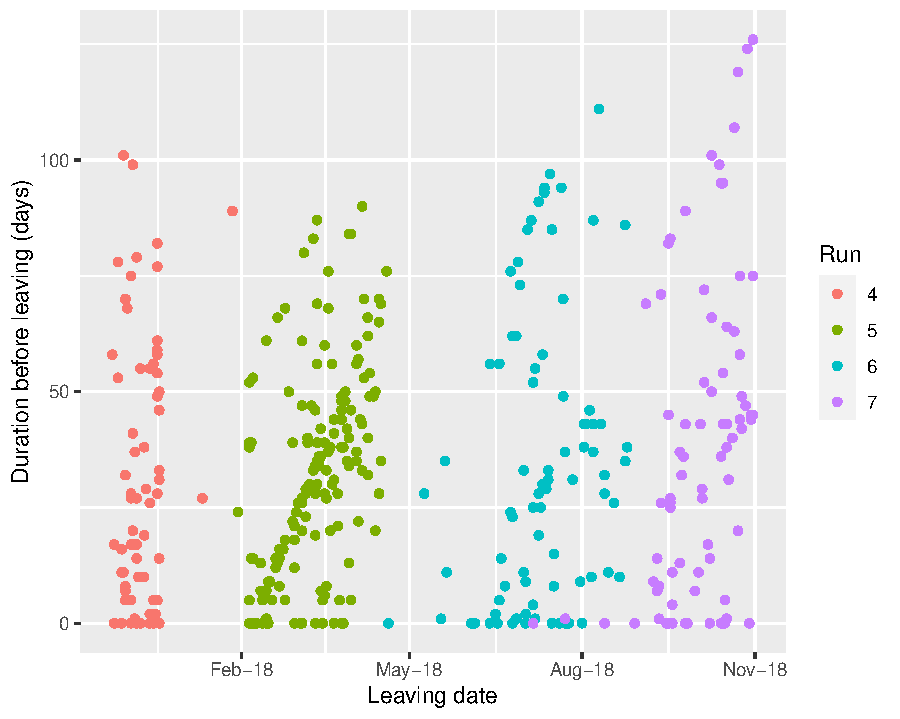
\includegraphics{report_files/figure-latex/unnamed-chunk-5-1} \end{center}

For graph 4, we will include the percentage of students who leave the
course in proportion to the overall enrollment for each run.

\begin{Shaded}
\begin{Highlighting}[]
\CommentTok{\# Insert plot 4}
\NormalTok{graph4}
\end{Highlighting}
\end{Shaded}

\begin{center}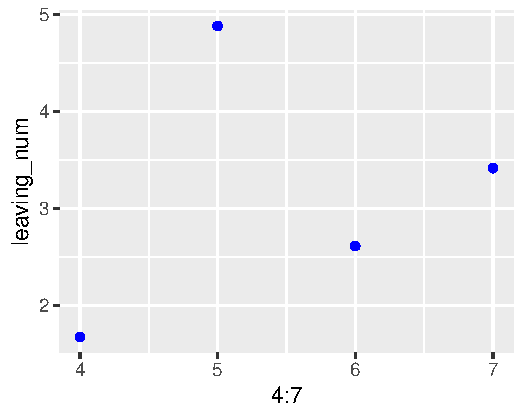
\includegraphics{report_files/figure-latex/unnamed-chunk-6-1} \end{center}

The last graph (graph 5) will present the bar plot consisting of the
number of entries for each reason.

\begin{Shaded}
\begin{Highlighting}[]
\CommentTok{\# Insert plot 5}
\NormalTok{graph5}
\end{Highlighting}
\end{Shaded}

\begin{center}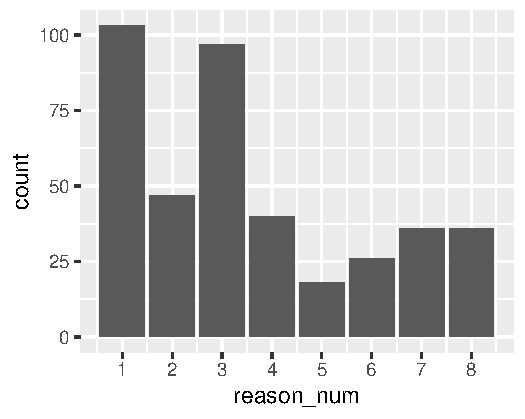
\includegraphics{report_files/figure-latex/unnamed-chunk-7-1} \end{center}

\hypertarget{discussion-1}{%
\subsubsection{Discussion}\label{discussion-1}}

In graph 3, we can see no distinct` patterns regarding either the
leaving date or the duration from starting to leaving. Students leaving
times are spread out evenly, just like the duration of quitting. Thus,
we can not extract any valuable insight from this graph. For graph 4,
the leaving rate of students (in proportion to the overall enrollments
number) ranges from 2\%-5\% and is also relatively low. Comparing graphs
2 and 4, the data suggest that many students dropped the class and did
not leave the course formally.\\
\hfill\break Graph 5 shows the bar plot consisting of the number of
entries for each reason. Each number represents the reasons below:

\begin{itemize}
\tightlist
\item
  I don't have enough time (1)
\item
  I prefer not to say (2)
\item
  Other (3)
\item
  The course required more time than I realised (4)
\item
  The course was too easy (5)
\item
  The course was too hard (6)
\item
  The course wasn't what I expected (7)
\item
  The course won't help me reach my goals (8)
\end{itemize}

\noindent We can see from the graph that the biggest reason for students
leaving the course is reason one, which is ``I don't have enough time.''
It then followed by reason three, ``Other'' and the other reason fairs
about the same. The high count of reason one suggests that many students
did not have enough time to learn and complete the course material. This
interpretation could be considered when designing the structure of
future course runs. The teaching and quiz interval could be made more
sparse, thus allowing more time flexibility for the students. Since many
students answered ``Other,'' it indicates that their reason for leaving
is not stated in the options above. Thus, to enable a more directed
feedback process in the future, more options should be listed, or
students should have the chance to write their reason for leaving
directly.

\hypertarget{question-3-1}{%
\subsubsection{Question 3}\label{question-3-1}}

\textbf{Which topic interests students the most?}\\
\hfill\break The video viewing status provided in the video-stats.csv
will determine which topic attracts students the most in the third
question. We will look at the variables total\_views and
viewed\_onehundred\_percent in detail. We will use the data we collected
in the previous phase to model the graph.\\
\hfill\break Graph 6 represents the variables
viewed\_onehundred\_percent against the step\_position. A different
colored line defines each run.

\begin{Shaded}
\begin{Highlighting}[]
\CommentTok{\# Insert plot 6}
\NormalTok{graph6}
\end{Highlighting}
\end{Shaded}

\begin{center}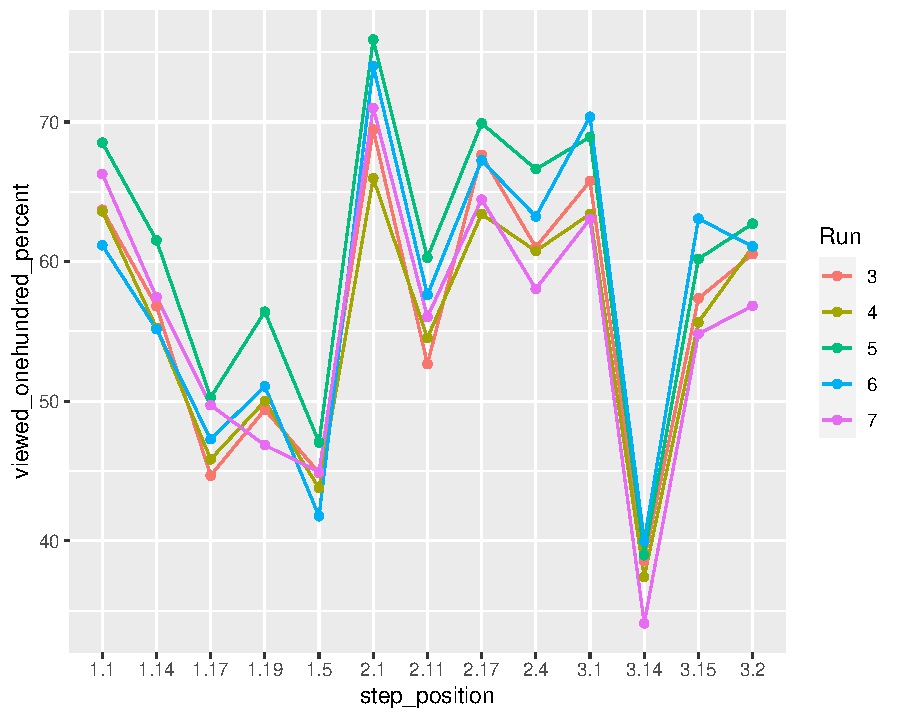
\includegraphics{report_files/figure-latex/unnamed-chunk-8-1} \end{center}

Similar to graph 6, graph 7 represents the variables total\_views
against the step\_position. A distinct colored line characterises each
run.

\begin{Shaded}
\begin{Highlighting}[]
\CommentTok{\# Insert plot 7}
\NormalTok{graph7}
\end{Highlighting}
\end{Shaded}

\begin{center}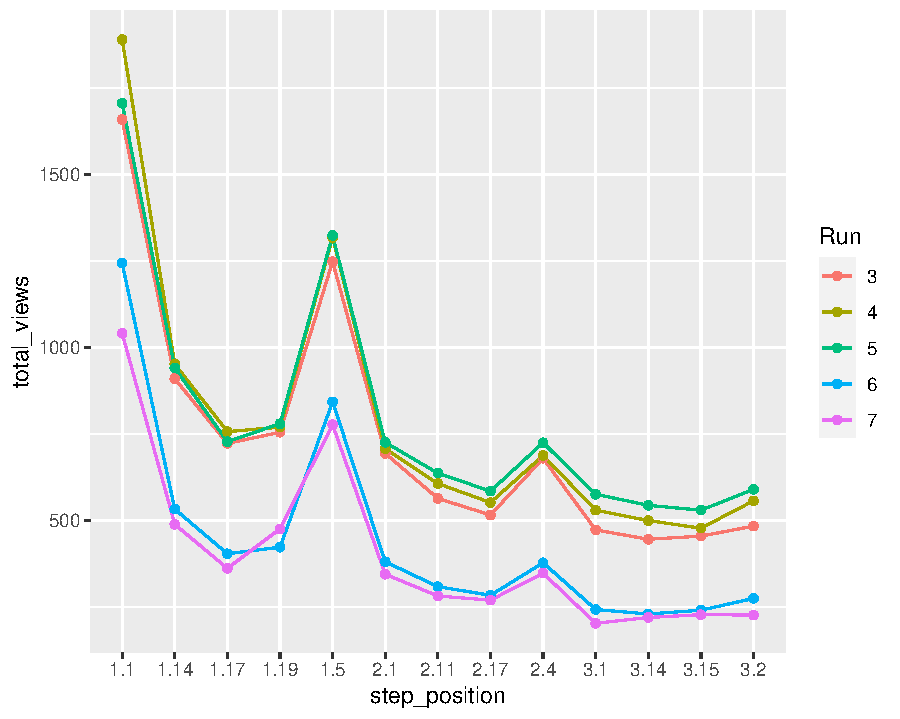
\includegraphics{report_files/figure-latex/unnamed-chunk-9-1} \end{center}

\hypertarget{discussion-2}{%
\subsubsection{Discussion}\label{discussion-2}}

In graph 6, we can see that each run peaks at step 2.1, which
corresponds to the topic of ``Welcome to Week 2: payment security''.
This interpretation suggests that those topics are the most engaging
ones for the student since many watched them until the end. For graph 7,
the highest peak is at the first video, corresponding to the topic
``Welcome to the course.'' The second peak is at step 1.5, corresponding
to the video ``Privacy online and offline.'' Overall, the trend of the
graph is decreasing. This analysis suggests that most of the students
are high-spirited at the beginning of the course, and their
participation decreases as time goes by. The plot also indicates that
the second peak topic, ``Privacy online and offline,'' catches the
students' attention the most. It is possible to elaborate more on the
issues mentioned above, payment security, and online or offline privacy
for future course runs.

\hypertarget{question-4-1}{%
\subsubsection{Question 4}\label{question-4-1}}

\textbf{Is there any correlation between the video views and the device
form?}\\
\hfill\break We used the cor function in the previous phase to check the
correlation between the number of views and the device form. The results
are as follow:

\tiny

\begin{Shaded}
\begin{Highlighting}[]
\NormalTok{cor\_res}
\end{Highlighting}
\end{Shaded}

\begin{verbatim}
##                           video_duration total_views viewed_onehundred_percent
## video_duration                1.00000000 -0.07226244               -0.55223027
## total_views                  -0.07226244  1.00000000                0.01969757
## viewed_onehundred_percent    -0.55223027  0.01969757                1.00000000
## desktop_device_percentage     0.05909484 -0.18405570               -0.50509760
## mobile_device_percentage     -0.20594228  0.96364814                0.20339651
## tablet_device_percentage      0.15528062 -0.96390169                0.02344017
##                           desktop_device_percentage mobile_device_percentage
## video_duration                           0.05909484               -0.2059423
## total_views                             -0.18405570                0.9636481
## viewed_onehundred_percent               -0.50509760                0.2033965
## desktop_device_percentage                1.00000000               -0.3725834
## mobile_device_percentage                -0.37258342                1.0000000
## tablet_device_percentage                -0.02729193               -0.9076307
##                           tablet_device_percentage
## video_duration                          0.15528062
## total_views                            -0.96390169
## viewed_onehundred_percent               0.02344017
## desktop_device_percentage              -0.02729193
## mobile_device_percentage               -0.90763066
## tablet_device_percentage                1.00000000
\end{verbatim}

\normalsize

\hypertarget{discussion-3}{%
\subsubsection{Discussion}\label{discussion-3}}

From the correlation result, we can see a strong positive linear
relationship between the total\_views and mobile\_device\_percentage.
This result suggests that most students watch the lecture video from
their mobile phones. Thus, video in the future could be made more
mobile-friendly. The correlation matrix also shows a positive
relationship between viewed\_onehundred\_percent with
mobile\_device\_percentage and tablet\_device\_percentage. This finding
indicates that students watching from their mobile or tablet devices are
more likely to finish their video than the other students watching from
the desktop. Other than that, the correlation matrix does not show any
other distinct patterns.

\hypertarget{deployment}{%
\section{Deployment}\label{deployment}}

For the deployment part, the user can access the whole process on the
following \href{https://github.com/c1040783/CSC8631}{Github repository}.
Additionally, this written final project will also be one of the
deployment forms since the user will understand and gain insight through
reading this.

\hypertarget{conclusion}{%
\section{Conclusion}\label{conclusion}}

In conclusion, we have completed the exploration process of a data
science project while adhering to the CRISP-DM methodology. We managed
to answer the questions imposed in the \emph{Business Understanding}
part with a coherent solution explained in the several phases. Resources
introduced in the course, such as library ggplot2 and dplyr, are also
used throughout the process.





\newpage
\singlespacing 
\bibliography{master.bib}

\end{document}